% ---------------------------------------------------------------------------
% PX915 individual project report -- Tristan McCarthy
% v2: condensed and restyled from report.tex (same data, equations and references).
% Build:  latexmk -pdf report_v2.tex     (REVTeX 4-2 + natbib, refs.bib)
% ---------------------------------------------------------------------------
\documentclass[aps,prb,twocolumn,superscriptaddress,floatfix,nofootinbib]{revtex4-2}

\usepackage{graphicx}
\usepackage{amsmath,amssymb}
\usepackage{booktabs}
\usepackage[dvipsnames]{xcolor}
\usepackage[colorlinks=true,allcolors=blue!60!black]{hyperref}
\usepackage{siunitx}

% Float placement: the defaults leave so little room per page that figures queue up and
% surface two pages after the text that cites them. These give LaTeX more freedom.
\renewcommand{\topfraction}{0.9}
\renewcommand{\bottomfraction}{0.7}
\renewcommand{\textfraction}{0.08}
\renewcommand{\floatpagefraction}{0.75}
\setcounter{topnumber}{3}
\setcounter{bottomnumber}{2}
\setcounter{totalnumber}{4}

\begin{document}

\title{Three-dimensional atom localisation with calibrated uncertainty from multislice
electron ptychography: mapping polar order in a PbTiO$_3$/SrTiO$_3$ superlattice}

\author{Tristan McCarthy}
\affiliation{HetSys Centre for Doctoral Training, University of Warwick, Coventry CV4 7AL, UK}
\author{Peng Wang}
\affiliation{Department of Physics, University of Warwick, Coventry CV4 7AL, UK}
\author{Nicholas D. M. Hine}
\affiliation{Department of Physics, University of Warwick, Coventry CV4 7AL, UK}

\date{\today}

\begin{abstract}
Polar vortices in ferroelectric superlattices are three-dimensional: the polarisation rotates
along the electron beam as well as across it, so a projection image integrates away the
structure it is used to measure. Multislice electron ptychography recovers depth from a single
orientation. Converting its phase volume into atomic coordinates is obstructed, however, by a
highly anisotropic response of $0.1$\,\AA{} in-plane against $1$--$2$\,\AA{} along the beam,
which buries the oxygen sublattice beneath its titanium neighbours. 4D-STEM of a relaxed
PbTiO$_3$/SrTiO$_3$ supercell was simulated, inverted, and every atom located by fitting the
volume as a superposition of a measured single-atom response. The method recovers $95.5\%$ of
bulk oxygen with $1.1\%$ species confusion, whereas three-dimensional deconvolution followed by
peak detection reaches at most $59\%$. That advantage is concentrated entirely in the axially
overlapped oxygen, for which recall is $82\%$ against $9$--$26\%$. Per-atom uncertainties combine
a joint Cram\'er--Rao bound with Mondrian conformal calibration, the former correcting the
twofold variance inflation a per-peak bound misses at the $1.95$\,\AA{} Ti--O spacing. The
resulting intervals hold their nominal coverage to within $1\%$ and transfer without retuning to
an independent reconstruction. Propagated through the Ti--O$_6$ off-centring, they yield the
local polarisation with error bars. The in-plane component is recovered to a median
$0.007$\,\AA{} and $0.9^\circ$, while the along-beam component is not determined, and that
conclusion is reached without reference to ground truth. Core-hole DFT indicates the missing
component remains spectroscopically accessible, the apical-oxygen O~K edge being $78\%$
dichroic to the polar-axis orientation with a monotonic $19\%$ arising from the displacement itself. Recovering
it would nonetheless require a collection aperture $\lesssim2$\,mrad rather than the
$100$\,mrad ptychography optics.
\end{abstract}

\maketitle
% ===========================================================================
\section{Introduction}
% ===========================================================================

Ferroelectric oxide superlattices host polar textures such as vortices, skyrmions and
labyrinths that have no counterpart in bulk ferroelectrics \citep{Yadav2016,Tang2015,Das2019,
Junquera2023}. In PbTiO$_3$/SrTiO$_3$ (PTO/STO), competition between elastic, electrostatic and
gradient energies drives the local dipoles into rotational arrangements whose topology, rather
than magnitude alone, is the property of interest. Establishing that topology requires the
measurement of a vector field at atomic resolution. The standard tool is atomic-resolution STEM,
in which the polarisation is inferred from the sub-\aa{}ngstr\"om offset of the B-site cation
from the centre of its oxygen cage, mapped column by column.

Such a measurement is a projection, and returns only the component of the off-centring lying in
the image plane. For a uniformly polarised domain this is minor and can be lifted by imaging a
second zone axis, but for a vortex it cannot, because the polarisation rotates with depth.
Different depths within one column then carry different, sometimes opposing, dipoles, of which
the image reports the average. The structure defining the texture is consequently the structure
the measurement removes.

Multislice electron ptychography (MEP) provides an alternative, reconstructing the specimen as a
stack of slices and thereby achieving optical sectioning from a single orientation
\citep{Gao2017,Chen2021,MaidenHumphryRodenburg2012}. Its lateral resolution is set by the
illumination angle rather than by the lens \citep{Nellist1995,Jiang2018,Nguyen2024}, and it has
been applied to dopant depths in bulk crystals \citep{Chen2021}, oxygen vacancy sites in
nickelates \citep{Dong2024} and, with a few coupled small-angle projections, to sub-nanometre
depth resolution \citep{Dong2025}. Atomic electron tomography offers quantified
three-dimensional coordinates \citep{Yang2017,Yang2021,Xu2015} but requires a large tilt series,
which is prohibitive for a beam-sensitive oxide.

The difficulty lies in what follows the reconstruction. A single-orientation measurement is
aperture-limited in depth, the lateral and axial resolutions scaling as $\lambda/2\alpha$ and
$\lambda/\alpha^2$, which for the $300$\,keV, $100$\,mrad probe used here are
$\approx0.10$\,\AA{} and $\approx2.0$\,\AA. Since the axial extent exceeds the $1.95$\,\AA{}
Ti--O spacing, an oxygen atom lies within the axial flank of its titanium neighbour and local
peak detection cannot separate the two. The established remedy of three-dimensional
Richardson--Lucy or maximum-entropy deconvolution followed by peak analysis \citep{Ishizuka2021}
was developed for sparse features rather than for a dense sublattice. The accepted
two-dimensional approach, model-based fitting of a peak superposition \citep{DeBacker2016},
does handle overlap explicitly, but it has not been extended to three dimensions for every atom
of a dense lattice simultaneously.

A second difficulty is more consequential for any physical conclusion. A polarisation map is a
difference of coordinates, each carrying an error, so whether a measured off-centring is real
cannot be judged without a per-atom uncertainty that is calibrated rather than merely reported.
Such uncertainties are rarely provided: a least-squares covariance is optimistic on
near-noiseless data, and the per-peak Cram\'er--Rao bound assumes all neighbours known exactly,
which is the assumption that fails on an overlapped lattice.

This work addresses both difficulties. 4D-STEM of a relaxed PTO/STO supercell was simulated and
reconstructed by MEP, and every atom was then located by fitting the phase volume as a
superposition of a measured single-atom response, which extends model-based quantification
\citep{DeBacker2016} to three dimensions and to all species simultaneously. Per-atom
uncertainties combining a joint Cram\'er--Rao bound with conformal calibration were attached to
those coordinates, shown to transfer to an independent reconstruction, and propagated into a
Ti--O$_6$ polarisation map. Core-hole DFT was then used to assess whether the component
inaccessible to ptychography is recoverable spectroscopically. Throughout, the localisation has
no access to the ground truth, which is used only to score the result.

% ===========================================================================
\section{Methods}
% ===========================================================================

\subsection{Model system}

\begin{figure*}[t]
  \centering
  
\includegraphics[width=0.70\linewidth]{figs/sample}\\[2pt]
  
\includegraphics[width=0.21\linewidth]{figs/tornado}
  \caption{The model system. (a) In-plane polarisation over the whole cell viewed down the beam,
    with one mean-direction arrow per atomic column, resolving the polar domains and vortices.
    The shaded square indicates the $20$\,\AA{} scan window and the shaded disc the exit-wave
    footprint spanned by the recorded diffraction, which is why the full box was simulated.
    (b) Atomic columns in beam projection within the scan region, with the overfocused probe
    ($\approx4$\,\AA) overlaid; the lead columns split into polar dumbbells. (c) Polarisation of
    the scanned volume in three dimensions, with the local dipoles (arrows, coloured by depth)
    twisting into a vortex tube along the beam. This depth variation is integrated away by a
    projection.}
  \label{fig:sample}
\end{figure*}

The test object was a relaxed atomistic supercell of a PTO/STO superlattice provided by
collaborators, of dimensions $70.0\times70.0\times47.9$\,\AA{} and containing $19\,440$ atoms,
comprising $1944$ formula units of each material. Both are perovskites (ABO$_3$), with heavy Pb
or Sr on the A site, Ti on the B site and oxygen on an octahedral cage; in the PTO layers the
B-site titanium and A-site lead are displaced from their centrosymmetric positions and the
resulting dipoles order into a labyrinth pattern. The local polarisation was quantified
throughout by the B-site off-centring
\begin{equation}
  \boldsymbol{\delta}_i \;=\; \mathbf{r}_{\mathrm{Ti},i} \;-\;
  \tfrac{1}{6}\!\!\sum_{j\in\mathrm{O}_6(i)}\!\!\mathbf{r}_{\mathrm{O},j},
  \label{eq:delta}
\end{equation}
the displacement of each titanium from the charge centre of its six nearest oxygens, mapped in
Fig.~\ref{fig:sample}(a).

The system is an exacting test of localisation for three reasons. The scattering contrast spans
two orders of magnitude, from lead ($Z=82$) to oxygen ($Z=8$), placing the light sublattice near
the noise floor, and the signal of interest is a sub-\aa{}ngstr\"om displacement of atoms
$1.9$--$3.9$\,\AA{} apart. The polarisation, moreover, twists with depth into a vortex tube
within the scanned volume (Fig.~\ref{fig:sample}c). The beam was set along a pseudocubic
$\langle100\rangle$ direction, giving a $\approx70$\,\AA{} path.

\subsection{4D-STEM simulation}

The simulation implements the forward operator $\mathcal{S}$ mapping the structure to the data a
microscope would record. A convergent probe of semi-angle $\alpha=100$\,mrad at $300$\,keV
($\lambda=1.969$\,pm) was focused $20$\,\AA{} above the entrance surface. It was then propagated
through the specimen by the multislice recursion \citep{CowleyMoodie1957,Kirkland2010}
\begin{equation}
  \psi_{n+1} = \mathcal{P}_{\Delta z}\!\otimes\!\big[\,t_n(\mathbf{r})\,\psi_n(\mathbf{r})\,\big],
  \qquad t_n = \exp\!\big[\,i\,\sigma\, v_n(\mathbf{r})\,\big],
  \label{eq:multislice}
\end{equation}
in which $v_n$ is the projected potential of slice $n$, $\sigma$ the interaction constant and
$\mathcal{P}_{\Delta z}$ the Fresnel propagator; the recorded quantity is
$I(\mathbf{r}_p,\mathbf{k})=|\mathcal{F}\psi_N|^2$. Calculations used abTEM
\citep{MadsenSusi2021} on GPU with Lobato potentials \citep{LobatoVanDyck2014}. Thermal motion
was included in the frozen-phonon approximation \citep{LoaneXuSilcox1991} as an incoherent
average over $16$ configurations, with amplitudes set per species from tabulated Debye--Waller
factors \citep{Peng1996}. Lead and oxygen vibrate roughly twice as far as titanium ($B=0.90$
and $0.80$ against $0.45$\,\AA$^2$), so a single averaged amplitude would misweight the diffuse
background of the species hardest to detect. A finite electron budget was imposed as shot noise,
$n \sim \mathrm{Poisson}(N_e\tilde I)$, over $D=10^{4}$--$10^{10}$\,e\,\AA$^{-2}$.

\subsection{Multislice ptychographic reconstruction}

Reconstruction inverts $\mathcal{S}$ by iterative ptychography
\citep{RodenburgFaulkner2004,Wakonig2020}, the single multiplicative projection being replaced
by a stack of $N_L$ transmission slices \citep{MaidenHumphryRodenburg2012}. Slices and probe
were recovered jointly by minimising the negative log-likelihood of the shot-noise model,
implemented as the variance-stabilised amplitude metric \citep{ThibaultGuizar2012} in the LSQ-ML
engine of \citet{Odstrcil2018} within PtychoShelves \citep{Wakonig2020}. Reconstructions used
$N_L=70$ slices (coherent, $\Delta z_{\mathrm{rec}}\approx1.0$\,\AA) or $105$ (thermally
averaged, $0.67$\,\AA). No regularisation was applied to the inter-layer coupling, so that the
axial structure is set by the data rather than by a smoothness prior, which would bias the
coordinate subsequently quantified. For the dosed data the illumination was treated as a mixed
state \citep{ThibaultMenzel2013} with orthogonal probe relaxation \citep{Odstrcil2016},
allowing the thermal diffuse background to be absorbed by incoherent degrees of freedom rather
than forced into the coherent object. Parameters are collected in Table~\ref{tab:params} of Appendix~\ref{app:params}.


\subsection{Atom localisation}
\label{sec:atomfind}

The reconstructed object was treated as a sparse superposition of identical single-atom
responses,
\begin{equation}
  \phi(\mathbf{r}) = \sum_{i=1}^{N} \beta_i\, K(\mathbf{r}-\mathbf{r}_i) + b(\mathbf{r})
  + \varepsilon(\mathbf{r}), \qquad \beta_i \ge 0,
  \label{eq:forward}
\end{equation}
in which $\phi$ is the per-layer median-subtracted phase, $(\beta_i,\mathbf{r}_i)$ the amplitude
and three-dimensional position of atom $i$, and $b$ a slowly varying background removed by a
high-pass filter. Since the reconstruction is a nonlinear inverse problem,
Eq.~\eqref{eq:forward} is an empirical linearisation rather than a derived identity, and is
tested directly in Sec.~\ref{sec:res-fwd}.

The kernel $K$ was measured rather than parameterised, a single isolated atom being propagated
through the byte-identical simulation and reconstruction pipeline and its reconstructed response
taken as $K$. This is necessary because $K$ is strongly anisotropic with an asymmetric axial
profile, so no simple parametric form is faithful. The lead kernel was used for all species,
since an isolated oxygen or titanium does not reconstruct above the noise floor; the response
shape belongs to the imaging system whereas the amplitude $\beta$ carries $Z$.

Estimation proceeds in two stages. The support is selected by matching pursuit on the dictionary
$\{K(\cdot-\mathbf{r})\}$ \citep{MallatZhang1993,Hogbom1974}, iteration being stopped at a
detection floor set relative to the local matched-filter noise rather than to an absolute phase
value, so that the threshold transfers between reconstructions of differing amplitude. The
support is then refined by block-coordinate descent, each atom being updated by Gauss--Newton
steps on the local residual with the current models of all other atoms subtracted, so that
overlap is accounted for to first order at every update. Candidates are retained on a
shape-based goodness-of-fit criterion rather than on amplitude, which preserves weak but
well-formed responses. The procedure extends model-based fitting of a peak superposition
\citep{DeBacker2016} to three dimensions with a measured kernel, applying to every atom of a
dense lattice a depth-from-axial-response estimate established for isolated dopants
\citep{Chen2021,Ishikawa2014}. Columns are then typed from their own fitted-amplitude
statistics, and sites predicted by a column's own periodicity but left empty by selection are
re-examined at a reduced threshold, such lattice-constrained detections being flagged so that
the constrained and unconstrained populations are reported separately. Thresholds, gates and
the full stage-by-stage specification are given in Appendix~\ref{app:algo}.

\subsection{Uncertainty quantification}
\label{sec:uq}

A model standard error, computed without ground truth, was separated from a calibration step
converting it into intervals with a stated coverage.

The model error has two terms, $\sigma^2=\sigma^2_{\mathrm{stat}}+\sigma^2_{\mathrm{sys}}$. The
statistical term is the Cram\'er--Rao bound of the \emph{joint} estimation problem, obtained by
assembling the Jacobian over all atoms in a subvolume and inverting the Fisher matrix once,
rather than the per-peak bound used to predict single-dopant precision
\citep{DeBacker2016,Chen2021}. On a dense sublattice the per-peak form is the bound obtained
with all neighbours known exactly, and is therefore optimistic by the variance inflation factor
of the overlapping templates. The systematic term $\sigma_{\mathrm{sys}}$ is the position spread
induced by kernel mismatch, which requires no ground truth and so transfers to experimental
data. Intervals were then obtained by split-conformal calibration
\citep{Vovk2005,AngelopoulosBates2023} in the Mondrian (label-conditional) variant
\citep{Vovk2003}, stratified by species, detection mode and depth band, so that coverage holds
per stratum rather than only on average. The $95\%$ interval is the default in released
coordinates, and the calibration table and per-stratum coverage are exported so that a dataset
on which the calibration fails to transfer is identified rather than trusted silently. The
derivation, the measured inflation factors and the coverage tables are given in
Appendix~\ref{app:uq}.

\subsection{Polarisation from located atoms}

Equation~\eqref{eq:delta} was evaluated on the located atoms exactly as on the model, the six
nearest located oxygens within $2.8$\,\AA{} forming the cage. Titanium whose cage is incomplete
in the reconstruction was excluded and reported separately rather than completed from the
lattice. Uncertainty on $\boldsymbol{\delta}$ was propagated by Monte Carlo, using $400$ draws,
from the per-atom conformal half-widths of Sec.~\ref{sec:uq}, that is from quantities available
without ground truth.

\subsection{First-principles EELS}
\label{sec:eels-method}

The energy-loss near-edge structure (ELNES) is governed by the dynamic form factor entering the
double-differential cross-section \citep{Egerton2011}. For the small momentum transfer
$\mathbf{q}$ of a near-axis collection, the dipole expansion gives
\begin{equation}
  S(\mathbf{q},E) \propto q^2 \sum_f
  \big|\langle f| \hat{\mathbf{q}}\cdot\mathbf{r}|i\rangle\big|^2\,\delta(E-E_f+E_i),
  \label{eq:dipole}
\end{equation}
so that the ELNES measures the symmetry-projected unoccupied local density of states along
$\hat{\mathbf{q}}$, which for a small on-axis aperture is essentially the beam direction, and in
an anisotropic crystal depends on its orientation relative to the polar axis
\citep{Nelhiebel1999}. The form of this expression frames the whole study. Since
$|\langle f|\hat{\mathbf{q}}\cdot\mathbf{r}|i\rangle|^2$ is even in $\mathbf{q}$, the dipole
ELNES is sensitive to the magnitude of the along-beam polarisation but not to its sign. A real
measurement, moreover, integrates over the convergence and collection apertures, and the
anisotropic term is weighted by a geometric factor vanishing at the magic angle
$\beta^\star\approx4\theta_E$, with $\theta_E=E/(\gamma m_0v^2)$ \citep{Jouffrey2004}.

Equation~\eqref{eq:dipole} was evaluated with CASTEP \citep{Clark2005} using the core-hole
method \citep{Gao2008}, in which the ionised atom carries an on-the-fly-generated
pseudopotential with one fewer core electron and a neutralising background, within a
$2\times2\times2$ supercell that dilutes the hole from its periodic images. The
core-to-conduction matrix elements were contracted by OptaDOS \citep{Morris2014,Nicholls2012}
into the core-loss spectrum with $\hat{\mathbf{q}}$ set explicitly. The central quantity is the
ELNES dichroism
\begin{equation}
  \Delta(E) = S(\mathbf{q}\!\parallel\!c,E) - S(\mathbf{q}\!\perp\!c,E),
  \label{eq:dichroism}
\end{equation}
which by reciprocity is the change in the measured edge when the polarisation rotates from along
the beam to in-plane. The O~K edge was taken as the primary observable, being an established probe of ferroelectric
off-centring \citep{TorresPardo2011,Bugnet2016}, while Ti~L$_{2,3}$ was treated for anisotropy
trends only, its $2p$ multiplet structure not being captured by single-particle DFT
\citep{Mizoguchi2009}. Calculations ran on the Warwick Blythe cluster, each core-hole SCF
requiring $40$--$45$\,min on $32$ cores and each OptaDOS pass $75$--$90$\,min.

% ===========================================================================
\section{Results and discussion}
% ===========================================================================

\subsection{The measured response and the forward model}
\label{sec:res-fwd}

\begin{figure*}[t]
  \centering
  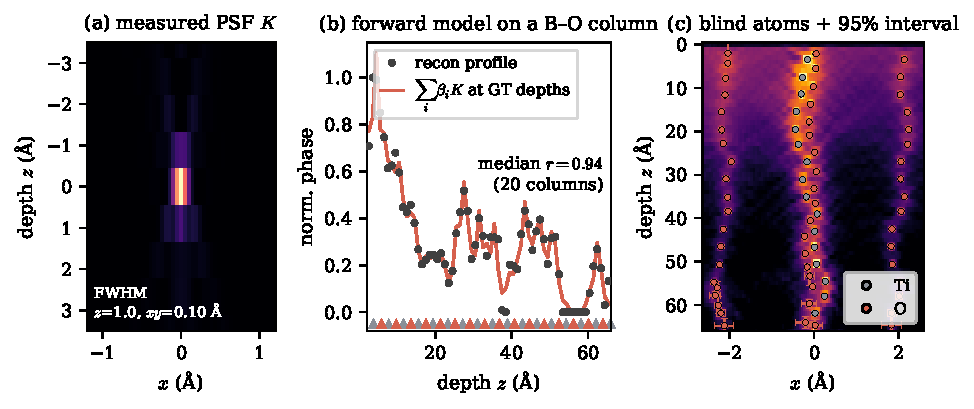
\includegraphics[width=\linewidth]{figs/fig_method}
  \caption{Model-based localisation. (a) The measured point-spread function $K$ in a depth--$x$
    slice, tight in-plane and elongated along the beam by the aperture-limited axial resolution
    of a single-orientation measurement. (b) Direct test of the forward model,
    Eq.~\eqref{eq:forward}: the measured depth profile of a mixed Ti--O column against the
    superposition $\sum_i\beta_iK$ of the measured response at the known atomic depths, matching
    at a median $r=0.94$ over $20$ columns. Triangles mark the true Ti (grey) and O (red)
    depths. The apparent $2$--$4$\,\AA{} axial blur is overlap of a fixed response rather than a
    loss of information. (c) Blind atoms located on a raw cross-section, coloured by assigned
    species, with calibrated $95\%$ intervals.}
  \label{fig:method}
\end{figure*}

The reconstructed single-atom response (Fig.~\ref{fig:method}a) has a full width at half maximum
of $0.10$\,\AA{} in-plane against $1.0$\,\AA{} along the beam for the coherent reconstruction and
$2.0$\,\AA{} for the thermally averaged one. Because that axial width is comparable to or larger
than the $1.95$\,\AA{} Ti--O spacing, neighbouring responses overlap and the design is not
separable. It is therefore necessary to establish whether the apparent blur represents overlap
of a fixed response or a genuine loss of information. Equation~\eqref{eq:forward} was tested by
fixing $\{\mathbf{r}_i\}$ at the known positions and solving for $\{\beta_i\}$ alone. A comb of
measured kernels at the true depths reproduces the observed depth profile of a mixed B--O column
at a median $r=0.94$ over $20$ columns (Fig.~\ref{fig:method}b), and $r=0.92$ in the full
depth--$x$ cross-section. The blur is consequently kernel overlap rather than lost information,
which is why a method that models the overlap can outperform one that does not.

\subsection{Localisation performance}

\begin{table}[t]
  \centering \small
  \begin{tabular}{@{}lccccc@{}}
    \toprule
    & \multicolumn{3}{c}{recall (\%)} & \multicolumn{2}{c}{oxygen split (\%)} \\
    \cmidrule(lr){2-4}\cmidrule(lr){5-6}
    method & Pb & Ti & O & isolated & overlapped \\
    \midrule
    3-D peak-pick, raw            & 93 & 88 & 72 & 91 & 26 \\
    RL deconv.\ $+$ peak-pick     & 93 & 87 & 58 & 79 & \phantom{0}9 \\
    MEM deconv.\ $+$ peak-pick    & 93 & 89 & 59 & 79 & 13 \\
    1-D per-column deconv.        & 91 & 65 & 49 & 62 & 20 \\
    3-D model fit                 & 88 & 89 & 89 & 92 & 82 \\
    \quad unconstrained only      & 88 & 89 & 86 & 92 & 71 \\
    \quad bulk, $z=10$--$56$\,\AA & 96 & 96 & 96 & --- & --- \\
    \bottomrule
  \end{tabular}
  \caption{Recovery of each sublattice, whole field unless stated, on the same reconstruction
    with the same measured kernel. Isolated oxygen occupies its own column; overlapped oxygen
    shares a column with titanium $1.95$\,\AA{} away. Precision is $0.97$ for the model fit
    ($0.98$ unconstrained) against $0.84$--$0.99$ for the baselines. Only the model fit returns
    species labels and per-atom uncertainties.}
  \label{tab:detect}
\end{table}

Table~\ref{tab:detect} scores the method against the known structure, alongside the established
alternatives run on the same volume with the same measured kernel, each at its own best-effort
threshold. Over the bulk ($z=10$--$56$\,\AA, excluding the entrance and exit artefact bands) the
model fit recovers $95.5\%$ of oxygen, $96.4\%$ of titanium and $95.6\%$ of lead, with $1.1\%$
of species labels incorrect, an in-plane RMS accuracy of $0.032$\,\AA{} and a depth RMS of
$0.37$\,\AA.

The aggregate oxygen figures understate what is being tested, so the sublattice was split by
geometry. Oxygen that is in-plane isolated, occupying its own column, is found by every method
at $79$--$92\%$. Oxygen that is axially overlapped, sharing a column with titanium
$1.95$\,\AA{} away, is the difficult case, and it is here that the methods separate: $82\%$ for
the model fit against $26\%$ for raw peak-picking, $13\%$ for maximum-entropy deconvolution and
$9\%$ for Richardson--Lucy. This population accounts for the whole of the advantage.

Neither of the remaining comparisons behaved as anticipated. Deconvolution before detection does
not assist, and Richardson--Lucy is actively detrimental to the oxygen, both routines losing
oxygen relative to peak-picking the raw volume at $58$--$59\%$ against $72\%$. They redistribute dynamic range
towards the strongly scattering species, so weak oxygen falls below any relative floor, and they
cannot restore the axial frequencies a single-orientation measurement never records, which are
precisely those separating an oxygen atom from the flank of its titanium neighbour. Ishizuka
\emph{et al.} report maximum entropy as the stronger routine \citep{Ishizuka2021}; no advantage
was reproduced on a dense lattice, so the limitation appears structural rather than a tuning
artefact. The second surprise is that on noiseless data a good peak-picker is competitive on the
heavy atoms, a raw local maximum being already a clean estimator of an isolated bright column. The margin quoted
here is consequently a lower bound, and the discriminating comparison is at finite dose
(Sec.~\ref{sec:dose}). A peak-picker cannot, at any dose, provide a species label or a
calibrated error bar.

\subsection{Calibrated uncertainty}

\begin{figure*}[t]
  \centering
  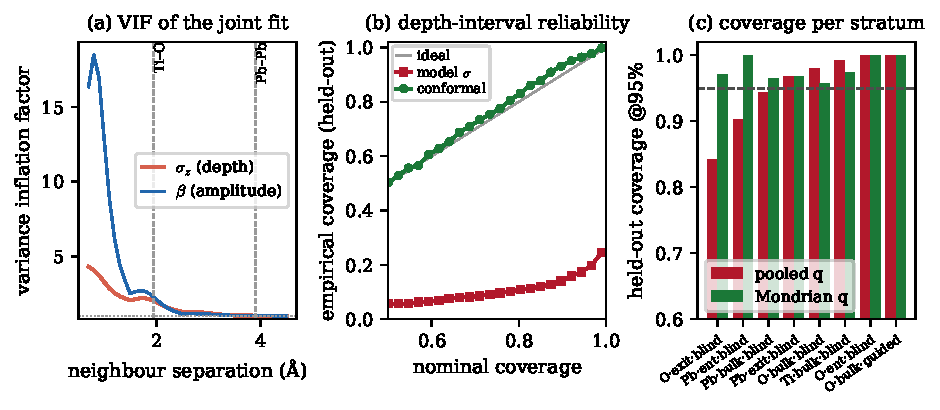
\includegraphics[width=\linewidth]{figs/fig_uncertainty}
  \caption{Calibrated uncertainty. (a) Variance inflation factor of the joint fit against
    neighbour separation: near unity at the $3.9$\,\AA{} heavy-atom spacing but ${\approx}2$ in
    depth, and larger in amplitude, at the $1.95$\,\AA{} Ti--O spacing, so that a per-peak
    Cram\'er--Rao bound is optimistic wherever responses overlap. (b) Held-out reliability of
    the depth interval: the raw model standard error treated as Gaussian (red) severely
    under-covers on near-noiseless data, whereas the conformal interval (green) tracks the ideal
    diagonal. (c) Held-out coverage at the $95\%$ level for the strata in which a single pooled
    quantile (red) departs most from target; the label-conditional quantile (green) restores
    coverage in each. Split-conformal, $50/50$ calibration/test split.}
  \label{fig:uq}
\end{figure*}

Figure~\ref{fig:uq}(a) quantifies why a per-peak bound is inadequate here. The variance
inflation factor of the joint fit is $1.04$ at the $3.9$\,\AA{} heavy-atom spacing, where atoms
are effectively independent, but $2.02$ in depth and $2.28$ in amplitude at the $1.95$\,\AA{}
Ti--O spacing, so that a per-peak bound understates $\sigma_z$ by $\approx1.4\times$ for every
apical oxygen. Since $85\%$ of atoms have a neighbour within $2.5$\,\AA, the per-peak form is
optimistic almost everywhere, and inverting the full Fisher matrix restores the inflation per
atom without a tuned constant.

The raw model $\sigma$ treated as Gaussian is nonetheless badly miscalibrated on near-noiseless
simulation, covering only $\approx8\%$ of atoms at a nominal $68\%$ (Fig.~\ref{fig:uq}b), since
the residual-based variance is near zero while the true error is dominated by systematics the
residual cannot detect. Conformal calibration supplies the missing scale empirically: held out
on a $50/50$ split, the interval tracks the ideal diagonal across the whole range of nominal
coverage, reaching $69/69/69\%$ in $(x,y,z)$ at a $68\%$ target and $96/96/96\%$ at $95\%$. The
Mondrian stratification is not cosmetic, the per-stratum quantiles $q_{68}(z)$ ranging from
$6.7$ to $14.4$, a factor of $2.2$, so that a single pooled constant leaves some strata
conservative
and others optimistic. In Fig.~\ref{fig:uq}(c) pooling drops the worst stratum to $84\%$ against
a $95\%$ target, whereas the label-conditional quantile restores every stratum to $95$--$100\%$.

The decisive test is whether an uncertainty estimate survives a change of dataset. The identical
code, with no tuned constants, was applied to an independent reconstruction of the same material
at a different in-plane sampling ($0.10$ against $0.15$\,\AA), a different slice discretisation
($105$ against $70$ layers), roughly half the phase amplitude and real reconstruction noise.
Re-running the conformal step on that volume's own atoms gives $69/69/69\%$ at the $68\%$ target
and $96/96/96\%$ at $95\%$. For comparison, the hand-tuned per-species error floors used in an
earlier version of this work, calibrated to $68\%$ coverage on the first volume, transferred to
$38/47/56\%$ on the second. The per-stratum quantiles on the harder volume span $10.9$ to
$23.3$, which is the regime a single floor cannot serve.

The scope of these intervals needs stating carefully. Each is conditional on the atom having
been correctly detected and typed, so that a spurious detection or species swap is a distinct
failure mode, reported separately as precision ($0.97$) and confusion ($1.1\%$). The exported species
posterior is a within-column amplitude confidence and is not itself calibrated, although labels
below $0.9$ are enriched for mislabelling by more than an order of magnitude over the base rate.
Finally, conformal calibration assumes exchangeability, which is why the workflow re-calibrates
per volume and exports the per-stratum coverage.

\subsection{Behaviour at finite dose}
\label{sec:dose}

\begin{table}[tb]
  \centering \small
  \begin{tabular}{@{}lccccc@{}}
    \toprule
    dose (e\,\AA$^{-2}$) & precision & Pb & Ti & O & confusion \\
    \midrule
    $10^{10}$ & 0.83 & 86\,\% & 74\,\% & 63\,\% & 13.7\,\% \\
    $10^{8}$  & 0.87 & 87\,\% & 72\,\% & 67\,\% & 11.8\,\% \\
    $10^{6}$  & 0.95 & 75\,\% & 25\,\% & \phantom{0}7\,\% & 38.0\,\% \\
    $10^{4}$  & ---  & \phantom{0}0\,\% & \phantom{0}0\,\% & \phantom{0}0\,\% & --- \\
    \bottomrule
  \end{tabular}
  \caption{Dose series on an independent reconstruction ($105$ layers, $0.10$\,\AA{} sampling),
    run with the same configuration as the coherent reference. The $10^{6}$ row illustrates the
    uninformativeness of precision. A guided-detection deduplication guard added subsequently
    reduces the $10^{10}$ confusion to $12.4\%$ with titanium recall unchanged.}
  \label{tab:dose}
\end{table}

Table~\ref{tab:dose} applies the same configuration over a dose series on the independent
reconstruction. Performance is maintained to $10^{8}$\,e\,\AA$^{-2}$ and collapses below
$10^{6}$. The residual gap to the coherent reference (Ti $74\%$ against $89\%$) is attributable
not to the localisation constants but to a harder reconstruction, having a $2.0$\,\AA{} axial
kernel against $1.0$\,\AA{} and a depth-registration correlation of $0.44$ against $0.63$.

The series carries a lesson that outlives this dataset. Precision is not a safety indicator: at
$10^{6}$\,e\,\AA$^{-2}$ it reads $0.95$ while titanium recall is $25\%$, oxygen $7\%$ and $38\%$
of labels are wrong, because it measures only the surviving bright lead atoms, which are
correctly placed. Species confusion and $\sigma$-coverage are the diagnostics that respond, and
both are printed as health warnings. Species assignment is coupled to depth registration as
well, since a $1$\,\AA{} depth error on a lattice whose Ti and O alternate every $1.95$\,\AA{}
swaps labels wholesale:
correcting the offset from $1.26$ to $0.29$\,\AA{} raised titanium recall from $53\%$ to $74\%$
and reduced confusion from $19.0\%$ to $13.7\%$ at $10^{10}$\,e\,\AA$^{-2}$. Sub-\aa{}ngstr\"om
depth accuracy is therefore a prerequisite for correct chemistry.

\subsection{Polarisation with error bars}
\label{sec:pol}

\begin{figure*}[t]
  \centering
  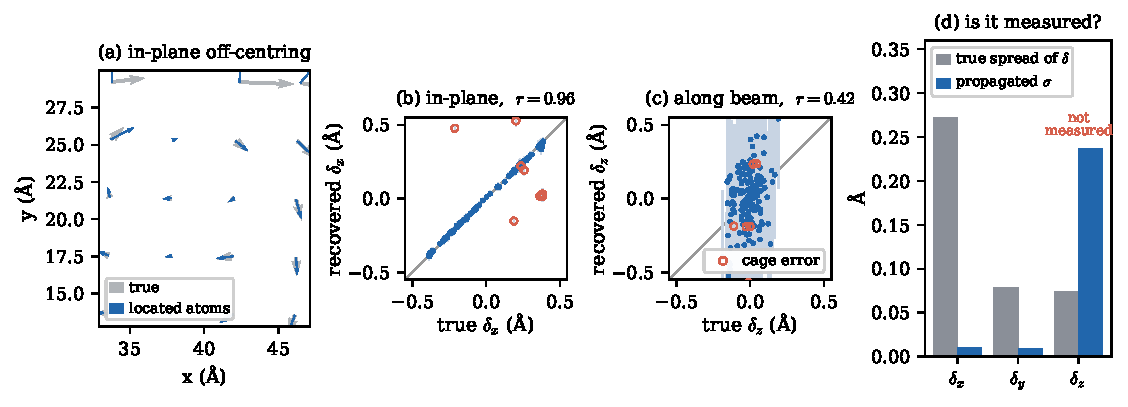
\includegraphics[width=\linewidth]{figs/fig_polarisation}
  \caption{Local polarisation from the located atoms. (a) In-plane Ti--O$_6$ off-centring
    averaged per atomic column: recovered (blue) over ground truth (grey). (b) Recovered against
    true in-plane off-centring, with propagated $95\%$ intervals; open red circles mark the
    $5\%$ of titanium whose oxygen cage has the wrong composition. (c) The same for the
    along-beam component. (d) Signal-to-noise per component, defined as the true spread of the
    component divided by the propagated $\sigma$ on it, on a logarithmic axis with the decision
    line at unity. In-plane the uncertainty is a small fraction of the signal, whereas along the
    beam it exceeds it, which is a ground-truth-free statement that the along-beam polarisation
    is not determined by this measurement.}
  \label{fig:pol}
\end{figure*}

Evaluating Eq.~\eqref{eq:delta} on the located atoms, $72\%$ of bulk titanium acquire a complete
oxygen cage from blindly located oxygens alone, of which $171$ match a ground-truth titanium and
are scored in Fig.~\ref{fig:pol}.

The in-plane off-centring is recovered essentially exactly. The median error in $\delta_x$ is
$0.005$\,\AA{} and in $\delta_y$ $0.004$\,\AA, against a true in-plane off-centring of mean
magnitude $0.274$\,\AA, for which the recovered mean magnitude is $0.273$\,\AA. As a vector it
has a median error of $0.007$\,\AA{} and a $90$th percentile of $0.017$\,\AA, while its
direction, the quantity from which a vortex map is constructed, has a median error of
$0.9^\circ$, with $95\%$ of titanium within $30^\circ$. The correlation between recovered and
true $\delta_x$ is $0.96$ over all matched atoms and $1.00$ once a small tail is excluded.

That tail requires comment. Five per cent of titanium have a cage of the wrong composition,
since a missing or misassigned oxygen displaces the centroid, and for these the in-plane error
rises to a median of $0.45$\,\AA, comparable to the signal itself. The propagated interval
covers $99\%$ of the well-caged titanium but only $12\%$ of the tail. This is not a failure of
the calibration but a statement of its scope: the interval is conditional on correct detection,
whereas a gross error in cage composition is a detection failure and must be reported through
precision, confusion and cage completeness rather than absorbed into a positional error bar. A
practical map should carry both, and the $28\%$ of titanium with incomplete cages should be
shown as absent rather than interpolated.

The along-beam component behaves in the opposite manner, and this is the more consequential
result. Its true spread across the scanned volume is small, $\sigma=0.074$\,\AA, since in this
zone axis the vortex polarisation is predominantly in-plane, whereas the propagated uncertainty
on $\delta_z$ is $0.237$\,\AA, more than three times the entire signal, and the correlation with
truth is correspondingly poor at $r=0.42$ with a median error of $0.122$\,\AA. The along-beam
component is therefore not measured by this experiment. The calibrated uncertainty establishes
this without ground truth, since comparing the propagated $\sigma_z$ with the spread of the
recovered $\delta_z$ requires no reference structure; it declares the along-beam map
uninformative while certifying the in-plane map to $0.01$\,\AA. Propagated intervals cover $95/93/99\%$ of
true errors in $(x,y,z)$ at a $95\%$ target, so neither the confidence in-plane nor the
pessimism along the beam is overstated.

Depth localisation of individual atoms is itself good, at $0.37$\,\AA{} RMS, comfortably better
than the $\approx2$\,\AA{} depth resolution, in the manner that single-molecule localisation
improves upon the diffraction limit \citep{Thompson2002}. A polarisation is, however, a
difference of two such coordinates, and differencing two $0.3$\,\AA{} depth errors cannot
resolve a $0.07$\,\AA{} displacement. In-plane the error is $0.03$\,\AA{} against a
$0.27$\,\AA{} signal, so the map is quantitative.

\subsection{Can EELS see the missing component?}

The second phase examines whether the along-beam polarisation leaves a spectroscopic signature,
and was constructed as a validated staircase. CASTEP/PBE reproduces the ferroelectric
instability: single-point energies across a displacement series $\mathbf{u}=s\,\mathbf{u}_0$ at
fixed tetragonal strain place the fully polar structure $203$\,meV per formula unit below the
centrosymmetric reference, monotonically, with the descent flattening towards $s=1$ so that the
experimental displacement lies at the PBE minimum. The core-hole recipe was fixed by reproducing
the rutile TiO$_2$ O~K ELNES, obtained with its textbook shape, the t$_{2g}$/e$_g$ near-edge
peaks split by $2.7$\,eV (experiment $2.5$--$3$\,eV) with $e_g>t_{2g}$. As an artefact check the
dichroism of the cubic cell at the isotropic Ti site is $0.02\%$, so any dichroism elsewhere is
physical rather than numerical.

\begin{figure*}[t]
  \centering
  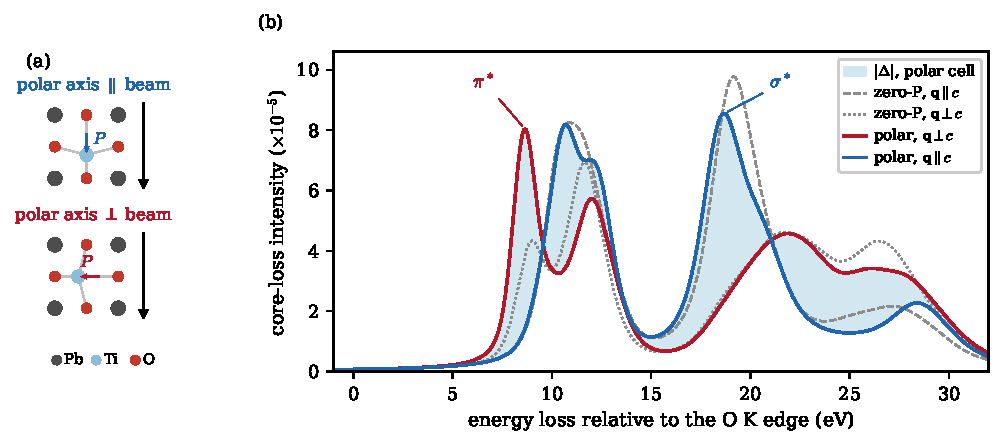
\includegraphics[width=0.74\linewidth]{figs/eels_dichroism}
  \caption{Orientation dichroism of the PbTiO$_3$ apical-oxygen O~K edge from core-hole CASTEP
    and OptaDOS.
    With the momentum transfer across the polar axis ($\mathbf{q}\perp c$, beam $\perp$
    $\mathbf{P}$) the edge shows a sharp $\pi^*$ peak; along it ($\mathbf{q}\parallel c$, beam
    $\parallel\mathbf{P}$) it shows the $\sigma^*$ features of the O~$2p_z$ states directed
    along the Ti--O--Ti chain. Grey curves are the same two orientations for the
    zero-polarisation, non-polar and equally strained reference, isolating the backbone
    contribution.}
  \label{fig:eels}
\end{figure*}

For the tetragonal cell with its polar axis along the beam, the apical-oxygen O~K edge is
strongly dichroic, with $\max|\Delta|/\max S = 78\%$ and $\int|\Delta|/\int S=47\%$ (Fig.~\ref{fig:eels}). The
origin is a $\sigma/\pi$ anisotropy: with $\mathbf{q}\perp c$ the edge shows a sharp $\pi^*$ peak
$\approx8.5$\,eV above onset from O~$2p_{x,y}$, whereas with $\mathbf{q}\parallel c$ it shows
$\sigma^*$ features at $\approx11$ and $18.5$\,eV from the O~$2p_z$ states directed along the
Ti--O--Ti chain. The excited site throughout is the apical oxygen, which lies on that chain
parallel to the polar axis. The O~K edge of the cell as a whole is the multiplicity-weighted sum
of one apical and two equatorial oxygen, and the equatorial calculation is outstanding, so the
values quoted here are those of the apical edge rather than of the weighted edge.

\begin{figure}[!htb]
  \centering
  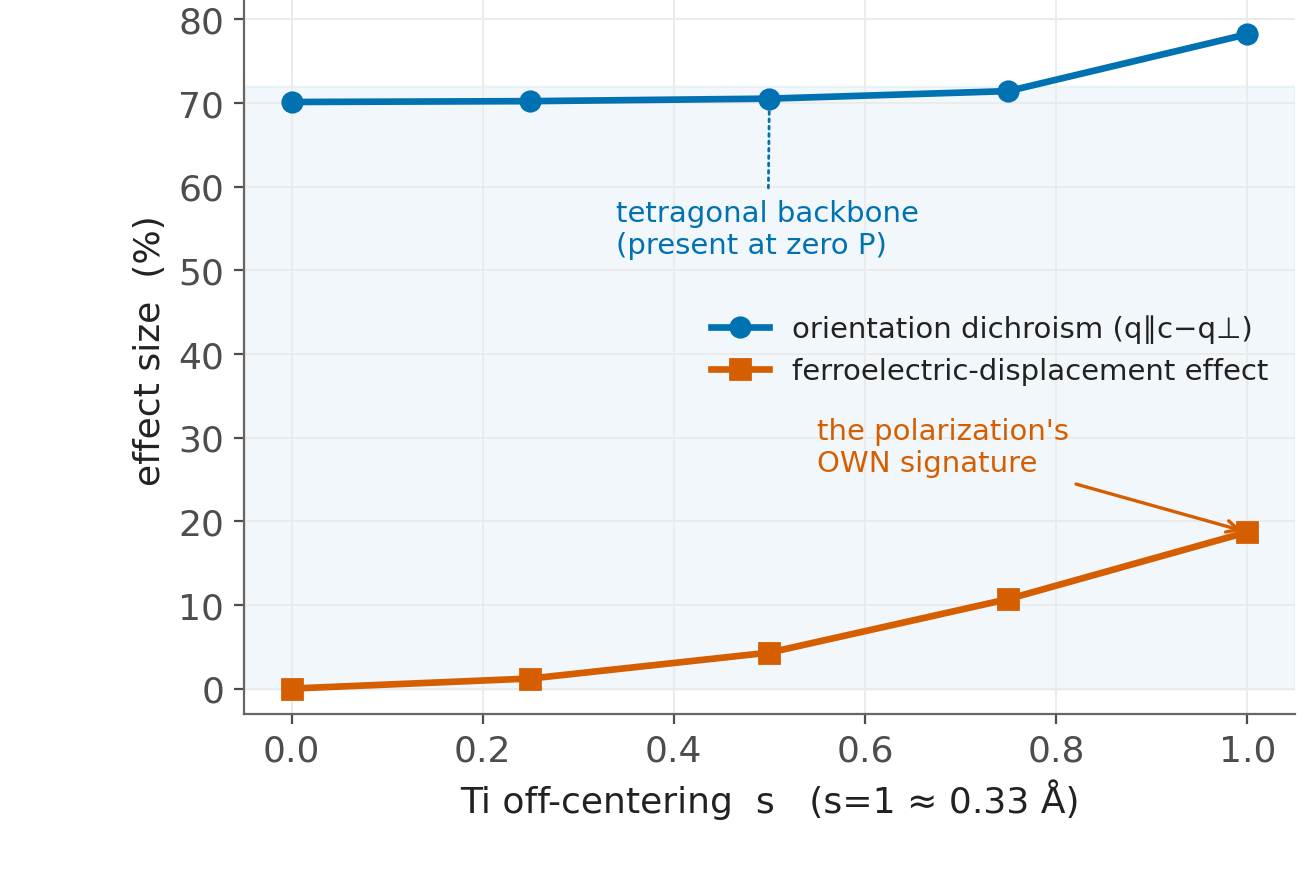
\includegraphics[width=0.92\linewidth]{figs/eels_decomp}
  \caption{Separating strain from polarisation. Holding the lattice parameters fixed and varying
    only the internal Ti off-centring $s$, the total orientation dichroism (blue) is already
    $70\%$ at zero polarisation, corresponding to the tetragonal backbone, whereas the signature
    of the ferroelectric displacement itself (orange) grows monotonically to $19\%$ at the
    experimental off-centring $|\mathbf{u}|\approx0.33$\,\AA.}
  \label{fig:eels-scan}
\end{figure}

A large orientation dichroism does not by itself constitute a polarisation measurement, since
the tetragonal backbone is anisotropic even without off-centring. Holding the lattice parameters
fixed and varying only the internal displacement $s$ separates the two contributions
(Fig.~\ref{fig:eels-scan}). At $s=0$, corresponding to zero polarisation with full tetragonal
strain, the dichroism is already $70.1\%$, rising to $78.2\%$ at $s=1$. Approximately $70$ of
the $78$ points are therefore the strain-induced backbone anisotropy, and the signature of the
off-centring itself is the remaining monotonic contribution: an $18.7\%$ change in the
along-beam-probed O~K spectrum between $s=0$ and $s=1$, $4.3\%$ at $s=0.5$, together with $8$
points of additional dichroism. This is the first-principles counterpart of the empirical
observation that the O~K edge responds to titanium off-centring \citep{Bugnet2016}, and it
renders the measurement a polarisation probe rather than merely a strain probe.

The intrinsic dichroism must then survive the acquisition geometry. For the O~K edge at
$300$\,keV, $\theta_E=1.09$\,mrad and the magic angle is $4.32$\,mrad $=3.98\,\theta_E$,
reproducing the textbook factor of $\approx4$ and validating the aperture model. Folding the
anisotropy through the collection geometry gives a surviving fraction of $0.62$ at
$\beta=1$\,mrad, $0.28$ at $2$\,mrad, $-0.04$ at $5$\,mrad and $-0.33$ at $100$\,mrad, so the
$100$\,mrad convergence of the ptychography probe averages the anisotropy away and indeed
inverts its sign. A combined ptychography and EELS experiment using one pixelated detector with
a central hole would collect at $\beta\approx100$\,mrad and would therefore suppress the signal
it was built to measure. Recovering the along-beam polarisation requires a dedicated aperture
$\lesssim2$\,mrad; at a $2\%$ fractional anisotropy this needs $\approx4.5\times10^{4}$ counts
per channel for SNR $3$, which sets the dose target.

Against this stand limits that no choice of aperture removes. The dipole ELNES is even in
$\mathbf{q}$, so it measures the magnitude of the along-beam polarisation but not its sign. A
dynamical multislice core-loss simulation of up- and down-polarised domains confirms as much,
the two giving O~K spectra identical to within $1.0\%$. In the labyrinth itself, viewed along
this zone axis, the polarisation is in any case mostly in-plane: over $2560$ polar titanium the
median angle from the beam is $82^\circ$
(interquartile range $73$--$87^\circ$), an along-beam fraction of only $\approx0.14$. The case
computed here is therefore an upper bound for this orientation.

% ===========================================================================
\section{Conclusions and further work}
% ===========================================================================

Fitting a reconstructed multislice-ptychographic volume as a superposition of a measured
single-atom response recovers the oxygen sublattice of a PbTiO$_3$/SrTiO$_3$ superlattice where
the established deconvolve-then-detect workflow does not, at $96\%$ bulk recall against at most
$59\%$. The whole of that margin lies in the axially overlapped oxygen ($82\%$ against
$9$--$26\%$). It is not a tuning artefact, since the limitation of deconvolution is the axial
spatial frequencies the aperture never records. The method also returns species labels ($1.1\%$
confusion) and calibrated per-atom uncertainty, neither of which a peak detector provides.

The uncertainty machinery is arguably the more transferable contribution. A joint
Cram\'er--Rao bound recovers the twofold variance inflation that a per-peak bound misses wherever
responses overlap, and Mondrian conformal calibration converts it into intervals holding their
nominal coverage per stratum. These contain no hand-tuned constant and transfer unchanged to an
independent reconstruction, on which hand-tuned error floors give only $38$--$56\%$ coverage
against a $68\%$ target. Reporting coverage rather than a fitted $\sigma$ is therefore to be
encouraged: the same pipeline that reads $\sigma$-calibrated at one dose reads $38\%$ species
confusion at another, while its precision still reads $0.95$.

Propagated into the physics, the result cuts both ways. The in-plane polarisation map is
quantitative, with a median error of $0.007$\,\AA{} in magnitude and $0.9^\circ$ in direction
against a $0.27$\,\AA{} signal. The along-beam component, by contrast, is not measured at all,
because differencing two $0.3$\,\AA{} depth coordinates cannot resolve a $0.07$\,\AA{}
displacement. The calibrated uncertainty establishes this without ground truth, which is the
purpose of such machinery. First-principles core-hole DFT indicates that the missing component is
spectroscopically accessible in principle, the apical-oxygen O~K edge being $78\%$ dichroic to
the polar-axis orientation, of which a monotonic $19\%$ is the signature of the displacement rather than of the
tetragonal backbone. The dipole limit nevertheless forbids recovery of the sign, and the magic
angle forbids use of the $100$\,mrad ptychography aperture for the purpose.

This leaves clear openings for further work. The assumption of one kernel for all species is
weakest where it matters most, since the larger Debye--Waller factor of oxygen broadens its
response under thermal scattering; in-situ vacancy-difference kernels would supply an in-crystal
oxygen matched filter. The $5\%$ cage-composition tail of Sec.~\ref{sec:pol} is a detection rather than a
localisation problem and requires a calibrated cage-completeness criterion, while learned
denoising before fitting \citep{Wu2026} is a natural route below $10^{6}$\,e\,\AA$^{-2}$. The
outstanding EELS cross-checks are the rotational-invariance test and the multiplicity-weighted
full O~K edge; beyond these, a faithful vortex simulation would inject a per-atom $\sigma(E)$
keyed to each oxygen's local polar-axis orientation. The clearest instrumental conclusion is a
design constraint, in that a combined depth-resolved-imaging and polarisation-spectroscopy
experiment cannot share one large aperture. The open question is whether the two can be fused into a
single three-dimensional vector polarisation measurement. Energy-filtered ptychography of the
oxygen sublattice \citep{Dong2024} and momentum-selective EELS of these flux-closure structures
\citep{Huang2026} both suggest routes.


\clearpage
\appendix
% appendix floats are numbered by their appendix letter (Table A1, C1, ...) so they are
% never confused with the main-text tables; the counter is reset in each appendix section.
\renewcommand{\thetable}{\thesection\arabic{table}}
\renewcommand{\thefigure}{\thesection\arabic{figure}}
\setcounter{table}{0}
\setcounter{figure}{0}

% ===========================================================================
\section{Simulation and reconstruction parameters}
\label{app:params}
\setcounter{table}{0}
\setcounter{figure}{0}
% ===========================================================================

Table~\ref{tab:params} collects the parameters of the forward simulation, the reconstruction and
the first-principles calculations. Reproducing the reconstruction from the simulated data
also depends on the geometry conventions recorded here. The object pixel is set by the
diffraction angle rather than by the scan step, giving $\mathrm{d}x=0.0492$\,\AA{} for the
binned $356^2$ detector, and the detector requires a single transpose relative to the
PtychoShelves convention. A two-stage
schedule, a down-sampled $178$-pixel pre-solve followed by a full-resolution $356$-pixel
refinement, accelerates convergence of the non-convex objective.

\begin{table}[t]
  \centering \small
  \begin{tabular}{@{}lll@{}}
    \toprule
    Stage & Parameter & Value \\
    \midrule
    Sample & composition & PbTiO$_3$/SrTiO$_3$, $19\,440$ atoms \\
           & supercell & $70.0\times70.0\times47.9$\,\AA \\
    \addlinespace
    Probe  & energy / $\alpha$ & $300$\,keV / $100$\,mrad \\
           & defocus & $-20$\,\AA{} ($20$\,\AA{} overfocus) \\
    \addlinespace
    Scan   & window / step & $20$\,\AA{} / $0.10$--$0.15$\,\AA \\
    \addlinespace
    Sim.   & slice thickness & $2.0$\,\AA{} ($0.5$\,\AA{} fine) \\
           & frozen phonons & $16$ configs; per-species $B$ \\
           & detector & $200$\,mrad, binned to $356^2$\,px \\
           & dose & $10^{4}$--$10^{10}$\,e\,\AA$^{-2}$ (Poisson) \\
    \addlinespace
    Recon  & engine & PtychoShelves LSQ-ML \\
           & layers $N_L$ & $70$ / $105$ ($\Delta z_{\mathrm{rec}}=1.0$ / $0.67$\,\AA) \\
           & regularisation & inter-layer off; $\beta_{\mathrm{LSQ}}=0.1$ \\
    \addlinespace
    DFT    & code / functional & CASTEP \citep{Clark2005} / PBE \\
           & core hole & full ($1s^1$/$2p^5$), charge $+1$ \\
           & supercell & $2\times2\times2$ (40 atoms) \\
           & spectra & OptaDOS \citep{Morris2014}, $\hat{\mathbf{q}}$-resolved \\
    \bottomrule
  \end{tabular}
  \caption{Simulation, reconstruction and first-principles parameters.}
  \label{tab:params}
\end{table}

% ===========================================================================
\section{Localisation algorithm}
\label{app:algo}
\setcounter{table}{0}
\setcounter{figure}{0}
% ===========================================================================

The five stages below operate on the reconstructed phase volume and the measured kernel alone.
No ground-truth quantity enters at any point.

\emph{Preprocessing.} Each layer has its median subtracted, so that vacuum maps to zero, and a
heavily Gaussian-blurred copy of the layer is removed to suppress the slowly varying channelling
haze that otherwise biases weak oxygen amplitudes. The result is clipped at zero and the
entrance and exit artefact layers ($z<2$\,\AA, $z>66$\,\AA) are trimmed.

\emph{Column seeding.} In-plane the problem is well conditioned, the kernel being two pixels
wide, so local maxima of the depth-averaged image over a $1.4$\,\AA{} non-maximum window give
$\approx98$ column seeds across the field.

\emph{Support selection.} Around each seed a fixed tube is taken, $\pm0.5$\,\AA{} in-plane and
spanning the full interior depth, and matching pursuit is run within it with the unit-norm
kernel: the residual is correlated with $K$, the global maximum is accepted as an atom,
$\beta K$ is subtracted, a neighbourhood of $\pm1.5$ layers by $\pm0.2$\,\AA{} is excluded, and
the process repeats. Iteration stops at $\max(K\star R)<k\,\sigma_{\mathrm{MF}}$, where
$\sigma_{\mathrm{MF}}$ is a median-absolute-deviation estimate of the matched-filter noise taken
over the sub-median voxels of the same tube and $k=2$. Because each atom carries its own
$(x,y,z)$, the ferroelectric lean of a column costs nothing.

\emph{Joint refinement.} Two sweeps of Gauss--Newton refinement follow. For atom $i$ the models
of all other atoms are subtracted and $(\beta,x,y,z)$ is fitted on the local patch by linearising
$K$, with $\partial K/\partial x$ and its counterparts obtained by central differences on the
measured kernel, giving sub-voxel positions. A candidate is rejected if the normalised
correlation between its patch and $\beta K$ falls below $0.5$. This is a shape test rather than
an amplitude cut, which matters because an amplitude cut cannot separate faint oxygen from
spurious detections whereas a shape test can.

\emph{Species assignment and lattice-constrained detection.} Columns self-classify by $k$-means
on their own per-column amplitude statistics, which are well separated in this material: the
$75$th percentile is $\approx4.1$ for lead columns, $\approx1.5$ for mixed B--O columns and
$\approx0.66$ for pure-oxygen columns, with no band overlap. On B--O columns titanium and oxygen
alternate every $\approx1.95$\,\AA, and species is assigned by per-column amplitude with a dead
zone, ambiguous atoms being resolved by local parity, that is by the distance of $z_i-z_j$
modulo the fitted period to confident neighbours. Parity is deliberately translation-invariant,
because a global comb phase accumulates period error towards the column ends and inverts labels
there. Expected sites are then enumerated by extending $\pm kp$ from each found atom of the same
species, and $\pm p/2$ from each titanium for oxygen; where a site is empty, meaning further
than $0.8$\,\AA{} from any same-species atom, a matched-filter search is run on the residual
within gates of $\pm0.7$\,\AA{} in depth and $\pm0.35$\,\AA{} in-plane, followed by refinement.
Such a detection is accepted only if its fit quality clears a reduced bar of $0.35$ and its
amplitude is lattice-consistent, lying between $0.45$ and $1.6$ times the column's same-species
median. The reduced bar is permitted for oxygen alone, the position prior substituting for the
missing contrast; the same treatment applied to lead and titanium produced mislocated atoms
with overconfident errors and was abandoned. A post-fit occupancy guard rejects any constrained
detection landing within $1.2$\,\AA{} of an atom already accepted in the same tube, no two atoms
in the reference structure being closer than $1.70$\,\AA. All such atoms carry a flag through to
the exported coordinates, so that the lattice prior is never silently absorbed.

% ===========================================================================
\section{Uncertainty quantification}
\label{app:uq}
\setcounter{table}{0}
\setcounter{figure}{0}
% ===========================================================================

\subsection{Joint versus per-peak Cram\'er--Rao bound}

For the stacked parameter vector $\theta=(\theta_1,\dots,\theta_N)$, with
$\theta_i=(\beta_i,\mathbf{r}_i)$, the Fisher information of Eq.~\eqref{eq:forward} under
homoscedastic residuals is $\mathbf{F}=\mathbf{J}^{\!\top}\mathbf{J}/s^2$, and the attainable
variance of $\theta_i$ is the corresponding diagonal block of $\mathbf{F}^{-1}$ rather than the
inverse of the diagonal block $\mathbf{F}_{ii}$. The two coincide only for an orthogonal design;
in general $[\mathbf{F}^{-1}]_{ii}\ge[\mathbf{F}_{ii}]^{-1}$, and the ratio is the variance
inflation factor (VIF) of the overlapping templates. Evaluating $[\mathbf{F}_{ii}]^{-1}$, in
which each atom is fitted with its neighbours held fixed, is the per-peak bound used to predict
single-column and single-dopant precision \citep{DeBacker2016,Chen2021}; on a dense sublattice
it is the bound obtained with all neighbours known exactly. Table~\ref{tab:vif} gives the
inflation measured for our kernel. Since $85\%$ of atoms in the field have a neighbour within
$2.5$\,\AA, the per-peak form is optimistic almost everywhere. We therefore assemble
$\mathbf{J}$ over all atoms in a subvolume and invert $\mathbf{F}$ once, a $4N\times4N$ system
with $N\le45$ and of negligible cost, taking each atom's marginal variance. This restores the
inflation per atom automatically and without a tuned constant.

\begin{table}[t]
  \centering \small
  \begin{tabular}{@{}llccc@{}}
    \toprule
    sep. & pair & VIF($\beta$) & VIF($z$) & $\sigma_z$ low by \\
    \midrule
    $3.90$\,\AA & Pb--Pb, Ti--Ti  & \phantom{0}1.04 & 1.04 & $\times1.02$ \\
    $1.95$\,\AA & Ti--O (apical)  & \phantom{0}2.28 & 2.02 & $\times1.42$ \\
    $0.99$\,\AA & near-degenerate & 13.3 & 3.33 & $\times1.83$ \\
    \bottomrule
  \end{tabular}
  \caption{Variance inflation of the joint fit relative to the per-peak bound, measured on the
    kernel used here. Every apical oxygen sits at the $1.95$\,\AA{} separation.}
  \label{tab:vif}
\end{table}

The systematic term $\sigma_{\mathrm{sys}}$ is obtained by generating a synthetic response with
one measured kernel, refitting it with another admissible kernel, and taking the resulting
position spread. Being computable without ground truth, it transfers to experimental data. On
the coherent reconstruction, where the lead and titanium kernels are nearly identical, it is
small ($\sigma_z=0.02$\,\AA); it grows on datasets whose kernels genuinely differ.

\subsection{Conformal calibration and measured coverage}

Nonconformity scores $s=|\Delta|/\sigma$ are formed per axis and the empirical $(1-\alpha)$
quantile taken with the finite-sample correction, the reported half-width being
$q_{1-\alpha}\sigma$. Coverage is guaranteed only marginally, and the error is strongly
heteroscedastic across the lattice, so calibration is performed per stratum, the strata being
species $\times$ detection mode $\times$ depth band. Table~\ref{tab:cov} gives the measured
held-out coverage on the coherent reconstruction and on the independent dosed volume. On the
latter the conformal step is re-run on that volume's own matched atoms, which is the intended
workflow, since applying one volume's quantile table to another assumes an exchangeability that
fails when registration quality differs. The per-stratum quantiles $q_{68}(z)$ span
$6.7$--$14.4$ on the coherent volume and $10.9$--$23.3$ on the dosed one, the wider spread on
the harder volume being precisely the regime a single floor cannot serve.

\begin{table}[t]
  \centering \small
  \begin{tabular}{@{}llcc@{}}
    \toprule
    volume & target & coverage $(x/y/z)$ & tuned floors \\
    \midrule
    coherent  & $68\%$ & $69/69/69\%$ & --- \\
    coherent  & $95\%$ & $96/96/96\%$ & --- \\
    dosed $10^{10}$ & $68\%$ & $69/69/69\%$ & $38/47/56\%$ \\
    dosed $10^{10}$ & $95\%$ & $96/96/96\%$ & --- \\
    \bottomrule
  \end{tabular}
  \caption{Held-out coverage of the calibrated intervals, split-conformal on a $50/50$ split.
    The final column gives the hand-tuned per-species error floors used in an earlier version of
    this work, calibrated to $68\%$ on the coherent volume and applied unchanged to the dosed
    one.}
  \label{tab:cov}
\end{table}

Exported per atom are the model $\sigma$, the $95\%$ conformal half-width taken as the default,
and a within-column amplitude posterior $p_{\mathrm{species}}$ for the assigned label. The last
is a relative confidence rather than a calibrated probability, and it is undefined in the useful
sense on single-species columns, but atoms with $p_{\mathrm{species}}<0.9$ are enriched for
mislabelling by roughly $25\times$ over the $1.1\%$ base rate.

% ===========================================================================
\section{Kernel provenance and noise robustness}
\label{app:kernel}
\setcounter{table}{0}
\setcounter{figure}{0}
% ===========================================================================

The kernel is measured by propagating a single isolated atom through the identical simulation
and reconstruction pipeline. Isolated light atoms do not survive this procedure: the titanium
and oxygen kernels extracted from the thermally averaged, dosed geometry have signal-to-noise
ratios of $2.4$ and $2.7$ respectively, with their interior maxima displaced to the volume
corner, and are unusable. The lead kernel of the coherent reconstruction is by contrast clean,
with a signal-to-noise ratio of $81.5$ and an axial full width at half maximum of $1.0$\,\AA,
and the corresponding thermally averaged lead kernel reaches $23.6$ at $2.0$\,\AA. A kernel
derived instead from lead blobs within the crystal is measurably worse, its axial width inflated
to $4.0$\,\AA{} by unresolved neighbours, and it reduces lead recall from $85\%$ to $65\%$. The
lead shape is therefore used for all species. The principal known limitation of this choice is
that the Debye--Waller factor of oxygen exceeds that of titanium ($B=0.80$ against
$0.45$\,\AA$^2$), so that under thermal scattering the true oxygen response is genuinely
broader than the lead response, and the assumption weakens exactly where it matters most.

Table~\ref{tab:noise} reports a controlled noise sweep in which Gaussian noise is injected into
the reconstructed volume with geometry, kernel and calibration held fixed. The intrinsic vacuum
noise floor of the volume is $\sigma\approx0.022$ and the oxygen peak amplitude
$\approx0.06$, so the collapse of oxygen recall between $\sigma=0.01$ and $\sigma=0.02$
corresponds to the oxygen signal falling below the noise. It is not a thresholding artefact and
no choice of detection floor removes it. The sweep also demonstrates the insensitivity of
precision as a diagnostic: at $\sigma=0.08$ the recall of both titanium and oxygen is zero and
three in four species labels are wrong, yet precision still reads $0.95$, because the surviving
bright lead atoms remain correctly placed. Species confusion and $\sigma$-coverage are the
quantities that respond, and the failure is at least conservative, the lattice-consistency
amplitude gate causing constrained oxygen detections to abstain rather than fabricate.

\begin{table}[t]
  \centering \small
  \begin{tabular}{@{}lcccccc@{}}
    \toprule
    injected $\sigma$ & found & precision & Pb & Ti & O & O overlapped \\
    \midrule
    0                 & 1834 & 0.97 & 88\,\% & 89\,\% & 89\,\% & 82\,\% \\
    0.01              & 1793 & 0.97 & 88\,\% & 91\,\% & 86\,\% & 74\,\% \\
    0.02              & 1421 & 0.98 & 87\,\% & 90\,\% & 57\,\% & 37\,\% \\
    0.04              & \phantom{0}795 & 0.96 & 87\,\% & 86\,\% & \phantom{0}5\,\% & 18\,\% \\
    0.08              & \phantom{0}408 & 0.95 & 87\,\% & \phantom{0}0\,\% & \phantom{0}0\,\% & \phantom{0}0\,\% \\
    \bottomrule
  \end{tabular}
  \caption{Injected-noise sweep on the coherent volume, all other settings fixed. Recalls are
    over the full depth rather than the bulk band. Species confusion rises from $1.1\%$ at
    $\sigma=0$ to $3.7\%$ at $0.02$, $58.7\%$ at $0.04$ and $74.6\%$ at $0.08$. The final column
    is the axially overlapped oxygen of Sec.~\ref{sec:bench}, the population on which the
    method's advantage rests, and it is also the population the noise removes first.}
  \label{tab:noise}
\end{table}

% ===========================================================================
\section{Reproducibility protocol}
\label{app:repro}
\setcounter{table}{0}
\setcounter{figure}{0}
% ===========================================================================

All code, the input structure and the per-run parameters are held in the project repository, the
pipeline being scripted end to end from simulation (\texttt{sim/simulate\_4dstem.py}) and
reconstruction (PtychoShelves \texttt{GPU\_MS}) through localisation
(\texttt{atomfind/run\_atomfind.py}) and polarisation (\texttt{atomfind/polarisation.py}) to the
DFT staircase (\texttt{eels/build\_cells.py}, \texttt{run\_coreloss.slurm},
\texttt{analyze\_elnes.py}), with a unit-test suite guarding structure generation and parsing.

\subsection{The nominated result}

The result offered for independent reproduction is the localisation-with-uncertainty output of
Sec.~\ref{sec:pol}. A peer receives three inputs: the reconstructed phase volume as a
$70\times404\times404$ complex array, the measured lead kernel, and the reference structure used
for scoring. The simulation and reconstruction that generate the volume require GPU resources
well beyond a few hours and are therefore supplied pre-computed; everything downstream of them
is reproduced from scratch. The two commands are
{\footnotesize\begin{verbatim}
python atomfind/run_atomfind.py \
       --preset NL70_coherent
python atomfind/polarisation.py
\end{verbatim}}
executed from the \texttt{analysis/} directory. The run requires a few minutes on a single core
and no GPU.

\subsection{Expected output and its uncertainty}

The first command writes \texttt{found\_atoms.csv}, containing for each atom its element, its
$(x,y,z)$ in \aa{}ngstr\"om in the reference frame, the per-axis $95\%$ conformal half-widths,
the model $\sigma$, the species confidence and a flag marking lattice-constrained detections,
together with the conformal quantile table. The second writes the Ti--O$_6$ off-centring with
its propagated uncertainty. On the same input the run is deterministic and should reproduce
$1834$ atoms with precision $0.97$, bulk recall $96/96/96\%$ for Pb/Ti/O, species confusion
$1.1\%$, in-plane RMS accuracy $0.032$\,\AA{} and depth RMS $0.37$\,\AA.

The uncertainty attached to each reported coordinate is the exported conformal half-width, and
the statement that validates it is the coverage figure itself: $96\%$ of true errors fall within
the nominal $95\%$ interval, per stratum, verified held out on a $50/50$ split
(Table~\ref{tab:cov}). Typical half-widths are $0.02$\,\AA{} in-plane and $0.5$\,\AA{} in depth,
rising to $1.5$\,\AA{} in depth for weak oxygen near the exit surface. Because they are strongly
heteroscedastic, the per-atom interval and not a global figure is the quantity to propagate. For
the derived polarisation the in-plane off-centring carries a propagated $\sigma$ of
$0.011$\,\AA{} and the along-beam component $0.237$\,\AA.

\subsection{Tolerances and known failure modes}

The single stochastic element is the conformal calibration split, which is seeded; re-seeding
changes the per-stratum quantiles by less than $5\%$ and leaves the coverage figures within one
percentage point. Coverage is a finite-sample quantity, so strata containing fewer than about
twenty atoms, of which the constrained-oxygen entrance band is the example here, show
conformal noise of several percentage points and should not be read as failures.

The scripts report their own failure modes rather than absorbing them, and a peer should expect
to see both. Approximately $28\%$ of bulk titanium do not acquire a complete oxygen cage, and
these are excluded from the polarisation map rather than completed from the lattice. A further
$5\%$ have a cage of the wrong composition, for which the in-plane error rises to a median of
$0.45$\,\AA{} while the positional interval covers only $12\%$ of them. This second mode is a
detection failure rather than a localisation failure, and is visible in the exported cage
completeness and species confidence rather than in the coordinate error bars.

\begin{acknowledgments}
The relaxed PbTiO$_3$/SrTiO$_3$ supercell was provided by collaborators and is used with their
agreement; we thank them for the structure. Calculations were performed on the Warwick Blythe
cluster and the Scientific Computing RTP. TM is supported by the EPSRC HetSys Centre for
Doctoral Training (EP/S022848/1).
\end{acknowledgments}

\bibliographystyle{apsrev4-2}
\bibliography{refs}

\end{document}
